Ein wesentlicher Teil dieser Arbeit besteht in der softwareseitigen Realisierung
der Laserstabilisierung und Experimentsteuerung. In diesem Kapitel sollen daher
alle Softwarekomponenten genauer betrachtet werden. Abschnitt
\ref{sec:datenerfassung_der_laser} wird beschrieben, wie die Informationen
der Laserfrequenzen aus der Counterkarte ausgelesen, im
Mikrocontroller \textit{Arduino} aufbereitet und anschließend am PC ausgewertet
werden. In Abschn. \ref{sec:stabilisierung_scan-strategie} wird die Regelung
der Laserfrequenz und der damit verbundenen Strategie der Frequenzverstimmung
erklärt. Abschnitt \ref{sec:linearisierung_iscan} beschäftigt sich mit der
Linearisierung der iScans und dem Neuschreiben der LUT. Die
Benutzerschnittstelle zur Experimentsteuerung soll in Abschn.
\ref{sec:experimentsteuerung} behandelt werden. In Abschn. \ref{sec:sonstiges}
werden weitere Funktionen kurz angerissen. Da die Software am PC in
Labview entwickelt wurde und somit der Code nur sehr platzverschwendend
dargestellt werden kann, wird die Beschreibung ausschließlich über
Ablaufdiagramme und Bildschirmfotos der Benutzeroberfläche geschehen. Der
Quellcode des Labview-Programms kann am Kontrollrechner selbst eingesehen
werden. Programme in Labview werden im Folgenden \textit{Virtuelles
Instrument} (VI) bzw. SubVI (Unterprogramm) genannt.

\section{Datenerfassung der Laser}\label{sec:datenerfassung_der_laser}
Die Informationen der Laser durchlaufen mehrere Stufen der Signal- und
Datenverarbeitung, bis eine quantitative Aussage über das Frequenzverhalten
gemacht werden und eine Regelroutine anlaufen kann. Der erste Teil der
Datenaufbereitung verläuft rein elektronisch, bis die Counterwerte binär in
den Counterregistern abrufbereit vorliegen, wie bereits in Abschn.
\ref{sec:elektronik_laserkontrolle} ausführlich erklärt wurde. An dieser Stelle
setzt nun die softwareseitige Weiterverarbeitung an. Im Folgenden wird sich
wieder exemplarisch nur auf einen Diodenlaser und den Referenzlaser bezogen.
Für alle anderen Laser gilt der identische Ablauf.

\subsection{Datenaufbereitung}\label{subsec:datenaufbereitung}
Zunächst werden die Counterwerte mit Hilfe des Mikrocontrollers \textit{Arduino}
ausgelesen und verarbeitet. Das komplette Ablaufdiagramm der Software des
\textit{Arduinos} ist in Abb. \ref{fig:ablaufdiagramm_arduino_laser} in auf die
wesentlichen Teile gekürzter Form zu sehen. Der komplette Quellcode hierfür
wurde in der Programmiersprache C geschrieben und ist im Anhang
\ref{anh:kap:quelltext_arduino_laserinformationsverarbeitung} zu finden.
\begin{figure}[hp]
 	\centering
 	\fbox{\parbox{\dimexpr \linewidth - 2\fboxrule - 2\fboxsep}{
 	\centering
	    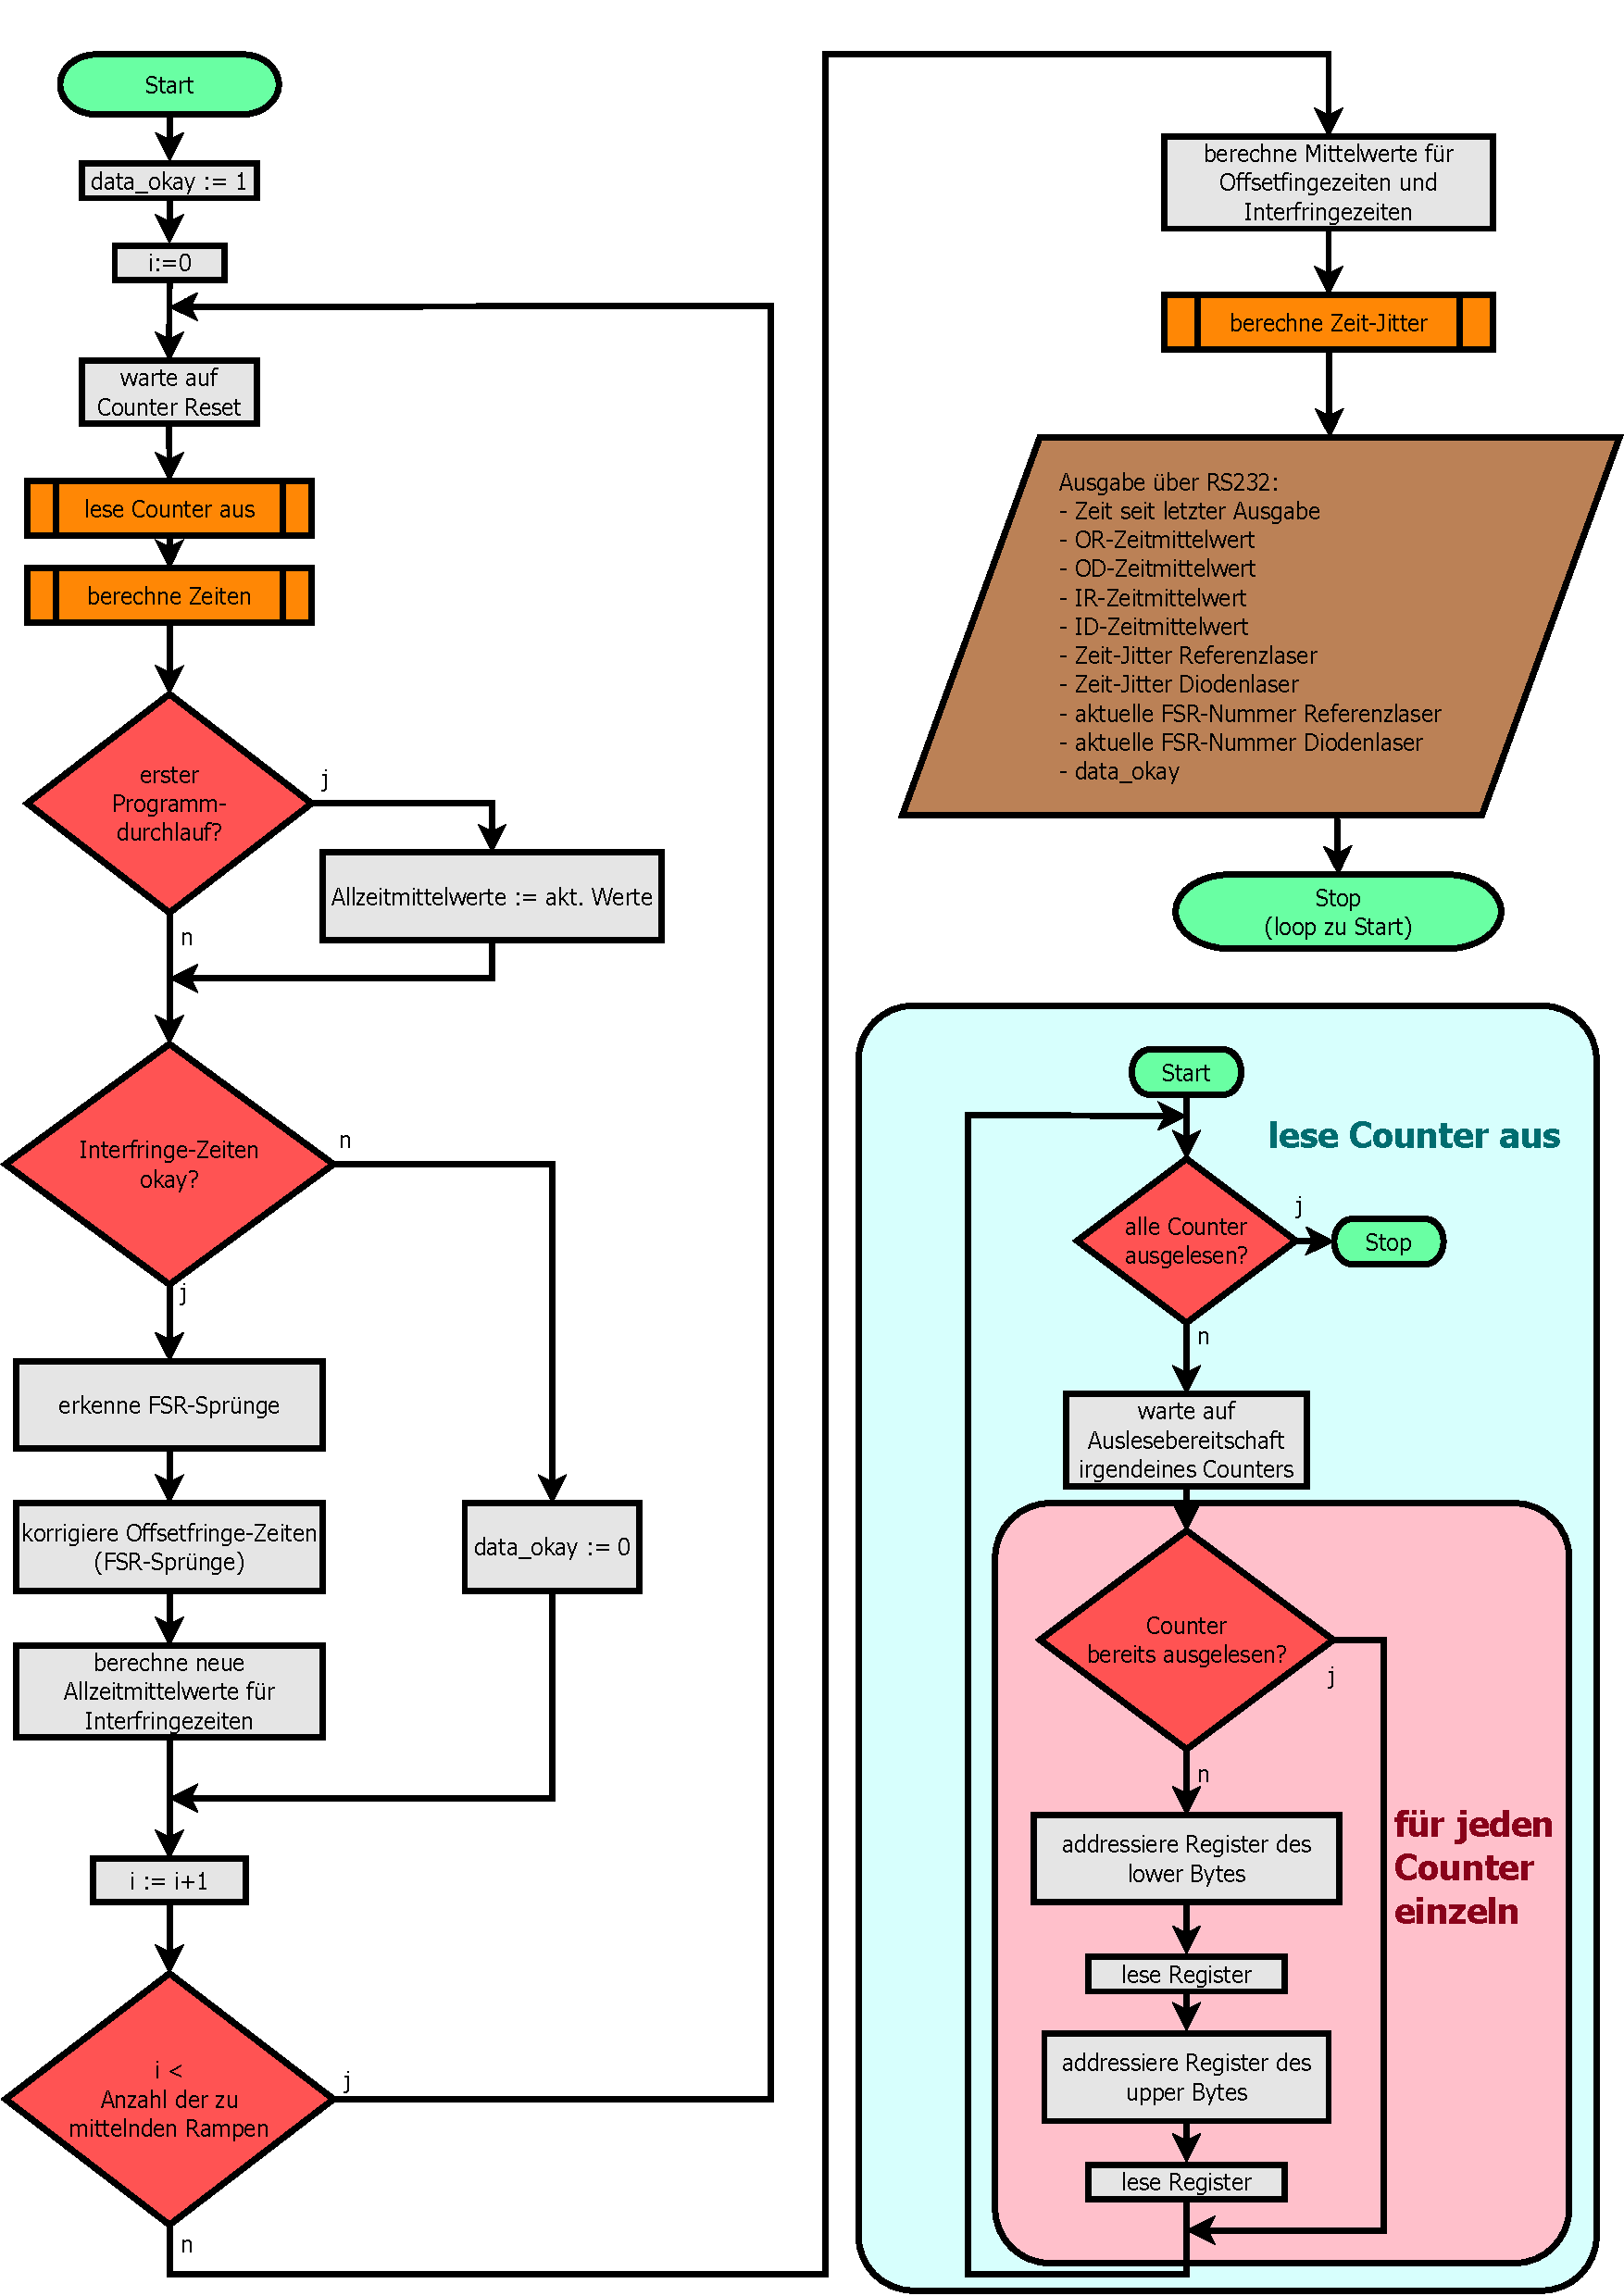
\includegraphics[width=\textwidth-0.5cm]{gfx/ablaufdiagramm_arduino_laser}
	    }}
	\caption[Laserdatenaufbereitung -
	Ablaufdiagramm]{Ablaufdiagramm der
	Laserdatenaufbereitung}\label{fig:ablaufdiagramm_arduino_laser}
\end{figure}
Der \textit{Arduino} verfügt über 54 digitale Ein- und Ausgänge, welche der
Kommunikation mit der Counterkarte dienen. HIGH ($5\,$V) bzw. LOW ($0\,$V) wird
als 1 oder TRUE bzw. 0 oder FALSE interpretiert. Das Programm besteht aus einem \textit{Setup}, in dem initialisierende Routinen wie die Pinbelegung
abgearbeitet werden, und einer \textit{Endlosschleife}
(\textit{Start}$\rightarrow$\textit{Programm}$\rightarrow$\textit{Stop}$\rightarrow$\textit{Start}$\rightarrow$\ldots),
über die die stetige Überwachung der Laser abgewickelt wird. Die Aufgaben des
Programms sind
\begin{itemize}
	\item Counter auslesen
	\item reale Zeiten berechnen
	\item unplausible Zeiten ignorieren
	\item FSR-Sprünge erkennen und Zeiten korrigieren
	\item Mittelwerte der Zeiten bilden.
	\item Laser-Jitter berechnen.
\end{itemize}
All dies muss innerhalb eines Rampenzyklusses (also innerhalb von maximal
$17\,$ms) geschehen, damit keine Information verloren geht. Im schlimmsten Fall
bleibt dem Mikrocontroller für die Berechnungen nach dem Auslesen der Counter
nur ca. $2\,$ms (fallende Rampe). Aus diesem Grund wurde das Programm möglichst
performand programmiert.\par Es wird immer eine bestimmte Anzahl von Rampenzyklen zusammengefasst und Zeitmittelwerte für die Offset- und Interfringezeiten beider Laser ($t_{OR,i}$,
$t_{OD,i}$, $t_{IR,i}$ und $t_{ID,i}$) berechnet. Weiterhin wird aus der
Standardabweichung der Offsetfringezeiten der Jitter
\begin{equation}\label{eq:jitter_zeit}
	\Delta
	t_O=\sqrt{\frac{1}{n-1}\cdot\sum\limits_{i=1}^{n}\left(t_{O,i}-\overline{t}_O\right)^2}
\end{equation}
des jeweiligen Lasers über die Anzahl der zu mittelnden Rampenzyklen
ermittelt.\par
Eine Iteration beginnt - wenn nötig - mit dem Warten bis alle
Counter zurückgesetzt wurden, indem geprüft wird, ob alle Status-Bits LOW sind, was irgendwann während der fallenden Rampe geschieht.
Anschließend werden die Counter ausgelesen. Dabei wird in einer Schleife zu
Beginn geprüft, ob bereits alle Counter ausgelesen worden sind. Wenn dies nicht
der Fall ist, wird über die Status-Bits auf die Bereitschaft irgendeines
Counters gewartet und im Falle der Bereitschaft geprüft, ob der Counter schon
ausgelesen worden ist. Wurden die Werte noch nicht ausgelesen, werden upper und
lower Byte nacheinander adressiert und ausgelesen.\par
Aus den erhaltenen 16-Bit-Werten werden nun über die fest einprogrammierte
Taktrate die wirklichen Zeiten berechnet. Über die komplette Zeit, in der das
Programm läuft, werden nach jeder Iteration Allzeitmittelwerte für die
Interfringezeiten erneuert. Zu Beginn des Programms werden diese mit den ersten
Zeiten initialisiert. Mit Hilfe der Allzeitmittelwerte wird geprüft, ob die
aktuellen Interfringezeiten valide sind. Es kann insbesondere bei schnellen
Frequenzverstimmungen vorkommen, dass während einer Rampe der Interfringe aus
dem aktuellen FSR hinausläuft, noch bevor der Counter gestoppt wurde und
somit eine falsche Zeit gemessen wird. Um diese Fälle und andere Fehlmessungen
auszusondern, wird geprüft, ob die gemessene Interfringezeit stark vom
Allzeitmittelwert abweicht.\par
Bei offensichtlich falscher Messung wird die
momentane Iteration abgebrochen und für die spätere Ausgabe ein
Validitätsvariable auf 0 gesetzt, damit bei der Weiterverarbeitung am PC
entschieden werden kann, ob die Daten genutzt werden möchten oder nicht. Sind
die Zeiten valide, kann herausgefunden werden, ob die Laserfrequenz einer der beiden Laser
in den nächsten FSR des FPIs gelaufen ist. Dabei wird jeweils überprüft, ob die
Zeit des Offsetfringes sich gegenüber der Zeit der vorherigen Rampe um mehr als
die Hälfte der Interfringezeit verändert hat. Gilt
$t_{O,akt.}-t_{O,alt}>\nicefrac{1}{2}\cdot t_{I,akt}$, so wird vermutet, dass
der Laser in den links benachbarten FSR gedriftet ist. Im Falle von
$t_{O,akt.}-t_{O,alt}<-\nicefrac{1}{2}\cdot t_{I,akt}$ ist der Laser vermutlich
in den rechts benachbarten FSR gedriftet. In beiden Fällen wird eine
FSR-Nummer-Variable erniedrigt bzw. erhöht. Die Detektion kann natürlich wie
schon erwähnt nur funktionieren, wenn die Frequenz deutlich langsamer als
$\nicefrac{1}{2}\text{FSR}$ pro Rampenzyklus verstimmt wird. Damit auch bei
FSR-Sprüngen die Zeiten zur Mittelung beitragen können, werden diese
anschleißend durch subtrahieren bzw. addieren der Interfringezeit
korrigiert.\par
Wurden genügend Rampen durchlaufen, können die aktuellen Mittelwerte aller
Zeiten und die Varianzen der Offsetfringezeiten berechnet und mit allen anderen
nötigen Werten über RS232 an den PC gesandt werden (brauner Kasten in Abb.
\ref{fig:ablaufdiagramm_arduino_laser}). Der String der versendet wird, beginnt
mit \lstinline|"*begin*"| und endet mit \lstinline|"*end*"|, damit später mit
sichergestellt werden kann, wo die Daten anfangen und aufhören. Die Werte sind
untereinander durch Leerzeichen getrennt.

\subsection{Datenbereitstellung am PC}\label{subsec:datenbereitstellung}
Die Daten eines jeden Lasers kommen wie oben erwähnt als String in Zeitabständen
eines Vielfachen der Rampendauer am PC an. Damit es zu keinem Pufferstau an
der seriellen Schnittstelle des PCs kommt, werden die aktuellen Strings direkt
nach Abschneiden von \lstinline|"*begin*"| und \lstinline|"*end*"| durch das
SubVI \lstinline|arduino_laser_read.vi| in globale Variablen geschrieben.
Parallel wird jeweils eine boolsche Variable gesetzt, die angibt, dass die Laserinformationen aktuell sind. Wird ein String aus einer der
globalen Variablen gelesen, wird die boolsche Variable zurückgesetzt und die
Laserinformationen werden als nicht mehr aktuell gewertet. Die aktuellen können
nun separat über das SubVI \lstinline|get_laser_times.vi| nach Angabe der
Lasernummer abgeholt werden. Das SubVI \lstinline|delta_time2delta_frequency.vi|
berechnet aus den Zeiten die Relativfrequenzen nach Gl.
\eqref{eq:FPI_frequenzdrift_03}. Das SubVI \lstinline|laser-control.vi|, die in
Abschn. \ref{sec:stabilisierung_scan-strategie} näher betrachtet wird, hat neben
der Regelung und Frequenzverstimmtung auf die Sollfrequenz auch die Aufgabe
Monitoringdaten an die Benutzeroberfläche der Laserkontrolle (Abb.
\ref{fig:benutzeroberflaeche_laserkontrolle}) weiterzugeben. Zu den
Monitoringdaten gehören Jitter des Lasers, Ist-Relativfrequenz und Abweichung
zur Soll-Relativfrequenz, wobei die detektierten FSR-Sprünge mit einbezogen
werden müssen. Die Referenzfrequenz ist beim Start des Programms oder beim
Drücken des Buttons \lstinline|assign| die derzeit aktuelle Laserfrequenz.
%TODO: !Screenshot: Laserkontrolle - Benutzerinterface

\section{Stabilisierung/Frequenzverstimmungs-Strategie}\label{sec:stabilisierung_frequenzverstimmungs-strategie}
